\section{Crypto-Predictive Markets}
\label{sec:crypto_predictive_markets}

The Crypto-Predictive Markets are a special type of decentralized finance where blockchain infrastructure is used to define smart contracts that can later be traded without the need for an intermediary, using some type of cryptocurrency as the exchange currency \parencite{HassanAmmar2023Fttt}. All transactions are recorded within the blockchain's ledger, being accessible to anyone who has a copy of the network. Additionally, there are special web browsers that allow viewing the records, filtering the information according to the user's needs. Below, we explore some basic concepts and how such infrastructure is employed in the context of predictive markets using Winner-Takes-All (WTA) type contracts.

\subsection{Basic Concepts}
\label{subsec:basic_concepts}

To understand the operation of a Crypto-Predictive Market, it is necessary to define some concepts that will later be used to describe how this infrastructure can be adapted in the context of WTA-type predictive market.

\subsubsection{Blockchain, Cryptocurrency and Layers}
\label{subsubsec:blockchain}

Commonly transactions are recorded in a ledger, which is an accounting book that records all transactions made. In the context of blockchain, this ledger is a distributed record among all the nodes of a network, which function as a redundant storage system. The term arises from the need to separate this record into blocks, in such a way that the handling of information is more efficient. Since the ledger or accounting book must be consistent throughout each block, they are chained together by a unique key called a hash.

In some blockchain protocols, layers are defined, so that the primary layer handles general records, while secondary layers handle specific records, which can be referenced from the primary layer without the need to record them directly. In the secondary layer, special rules can be defined for the management of records, such as the definition of a smart contract.

The process of recording a block in the ledger requires that a unique key be generated to chain the blocks. This generation of keys is not automatic, but requires the computation of keys through computational power. Different blockchains implement tokens called cryptocurrencies, which are used as rewards for the nodes that perform the computation of the keys. This process is called mining, and it is the way in which the consistency of the ledger is maintained throughout the network. Because the records in the ledger can represent real transactions, there is a monetary equivalence for cryptocurrencies, due to the added value of recording the transaction.

\subsubsection{Smart Contracts}
\label{subsec:smart_contracts}

A smart contract is a program embedded in the secondary layer of the blockchain. This contract contains the rules and deadlines that will enforce the promise of an agreement between two or more parties. These contracts do not require a legal intermediary to mediate between the parties, and the defined execution conditions are validated by a network of specialized agents known as oracles \parencite{alma9919406254106531}.

\subsubsection{Oracles}
\label{subsubsec:oracles}

Smart contracts typically establish execution conditions that require information not recorded within the blockchain. The inclusion of such external information and its tracking within the blockchain is not efficient, so a solution to this problem is to use agents that follow and validate the external information. When the contract's execution condition is met, these agents inform the contract that the condition has been fulfilled, and through a voting system, a consensus is reached among information validating agents as to whether the condition was met or not. These agents are called oracles \parencite{HassanAmmar2023Fttt}.
    
Oracles can be human agents or programs external to the blockchain. To validate a contract's condition, oracles must stake a certain amount of money, usually in the form of cryptocurrencies. Those who correctly validate the information receive a reward, while those who do not lose the money staked.
    
The more oracles a smart contract has, the more robust the results will be, and the lower the probability that a malicious oracle can alter the outcome. The number of oracles needed depends on the nature of the contract. For example, the outcome of an official Champions League football match may require few oracles, with applications connected to official information sources. On the other hand, validating hypotheses or opinions may require a larger number of oracles, due to the inherent subjectivity of the information.

\subsection{Crypto-Predictive Markets}
\label{subsec:crypto_predictive_markets}

In a Crypto-Predictive Market, a smart contract is used to define the rules of a market, setting the conditions under which a market is considered resolved. Agents can participate in the market, buying and selling shares according to their beliefs. When the market is resolved, those agents who bought shares in accordance with the correct outcome receive a reward, while those who bought shares based on an incorrect outcome lose the money staked. Oracles are used to validate the outcome of this market, which, according to the terms defined in the smart contract, receive a reward or are penalized for the correct or incorrect validation of the contract's execution condition.
    
A special type of contract is the Winner-Takes-All (WTA). In the context of a smart contract, this specific type uses a binary execution condition, either fulfilled or not fulfilled. The price of the shares is set between 0 and 1, and those agents who bought shares according to the correct outcome receive a reward of 1, having a gain of $1-p$, where $p$ is the price at which they bought the share.

\subsection{Polymarket}
\label{subsec:polymarket}

Polymarket is a web platform that facilitates the participation of agents in markets defined through smart contracts. The platform is merely an interface where agents can interact with the smart contracts defined on Polygon, a blockchain that operates on the secondary layer of Ethereum, designed to facilitate the creation and management of smart contracts \parencite{PolymarketLearn}.

In Figure \ref{fig:polymarket}, an example of a predictive market on the Polymarket platform can be seen. It shows the main elements which are: \begin{enumerate*}[label=(\roman*)]
\item the name of the market,
\item the conditions under which the market is considered resolved,
\item the information source that the oracles will consult,
\item the date on which the market closes,
\item the total amount of bets measured in dollars, and
\item the price of the long and short positions.
\end{enumerate*}

\begin{figure}[htbp]
    \centering
    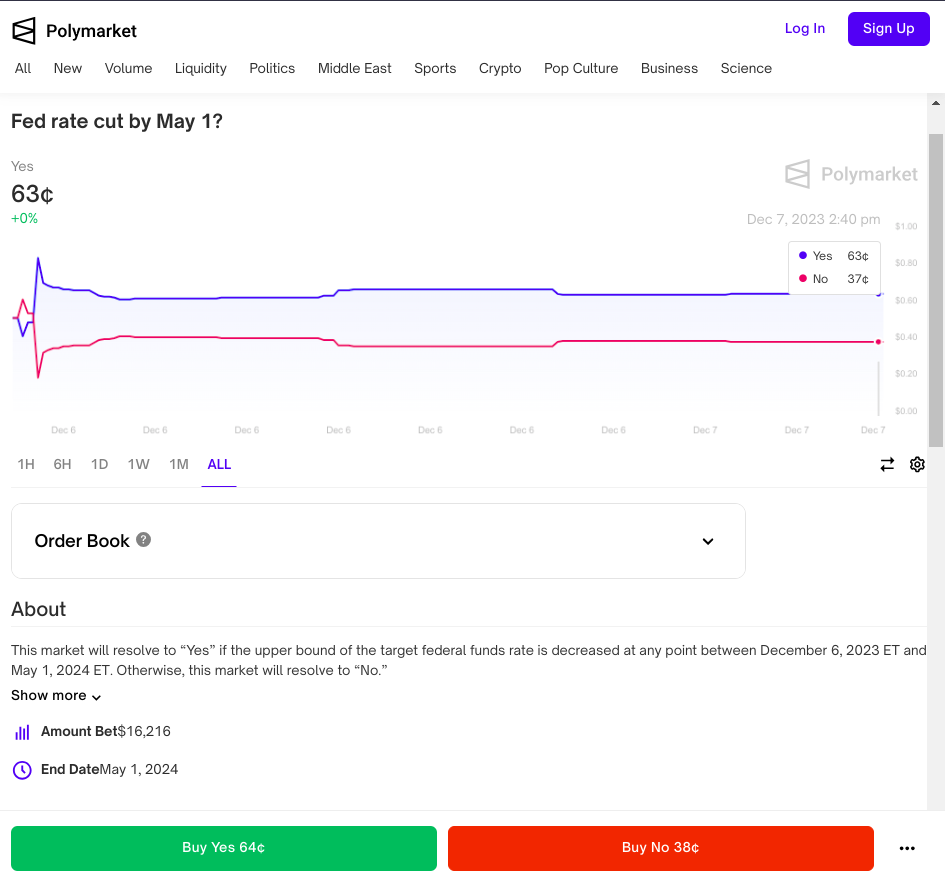
\includegraphics[scale=0.4]{img/polymarket.png}
    \caption{Polymarket Platform}
    \label{fig:polymarket}
\end{figure}

In these markets, the long position represents those agents who believe that the market will resolve as true, while the short position represents those agents who believe the opposite. In Figure \ref{fig:polymarket}, the long position (indicated in green) represents those agents who expect the FED to cut interest rates by May 2024, while the short position (indicated in red) represents those agents who expect the FED not to cut interest rates for the same date.
    
The price of the long and short positions add up to one, and the interpretation of this price is the probability that agents assign to the market resolving as true or false. In Figure \ref{fig:polymarket}, the price of the long position is 0.63, which means that the aggregated probability of agents expecting the FED to cut interest rates by May 2024 is 63\%. Complementarily, the price of the short position is 0.37, which means that the aggregated probability of agents expecting the FED not to cut interest rates by May 2024 is 37\%.

\subsubsection{Supply and Demand Mechanism}
\label{subsubsec:supply_and_demand_mechanism}

The price of the long and short positions is determined through a supply and demand mechanism. This mechanism is recorded in the Order Book.

\begin{figure}[htbp]
    \centering
    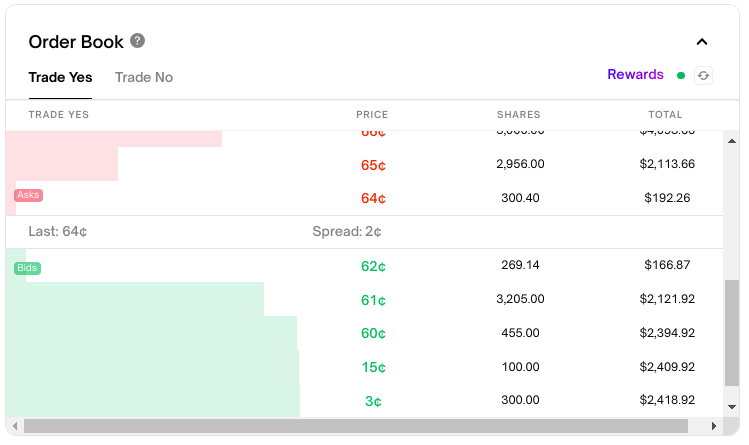
\includegraphics[scale=0.4]{img/order_book_yes.png}
    \caption{Order Book for the Long Positon}
    \label{fig:order_book_yes}
\end{figure}

In Figure \ref{fig:order_book_yes}, the Order Book for the long position can be observed. In the center, the last transaction made is shown, which determines the current price. In the upper part (called Ask), all the agents willing to sell their long positions at a certain price are listed, and in the lower part (called Bid), all the agents willing to buy long positions are found. In the order book only the unrealized orders are shown, that is, those orders that have not been matched. When an order is matched, the transaction is recorded in the blockchain, and the order is removed from the order book.
 
\begin{figure}[htbp]
    \centering
    \begin{minipage}{.5\textwidth}
        \centering
        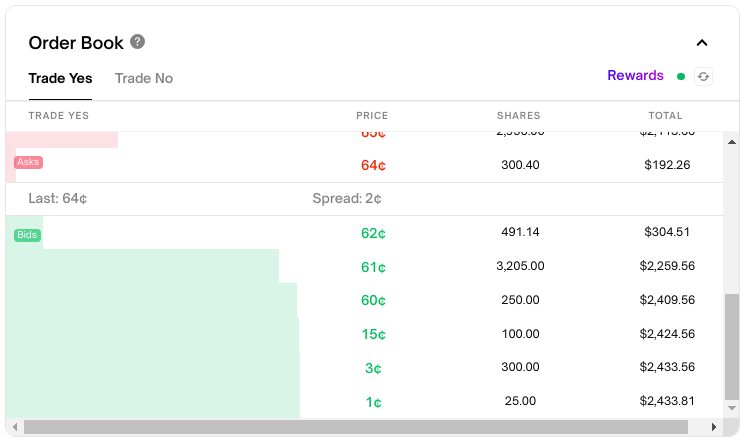
\includegraphics[scale=0.3]{img/order_book_yes_bid.png}
        \caption{Order Book for the Long Position: Bid}
        \label{fig:order_book_yes_bid}
    \end{minipage}%
    \begin{minipage}{.5\textwidth}
        \centering
        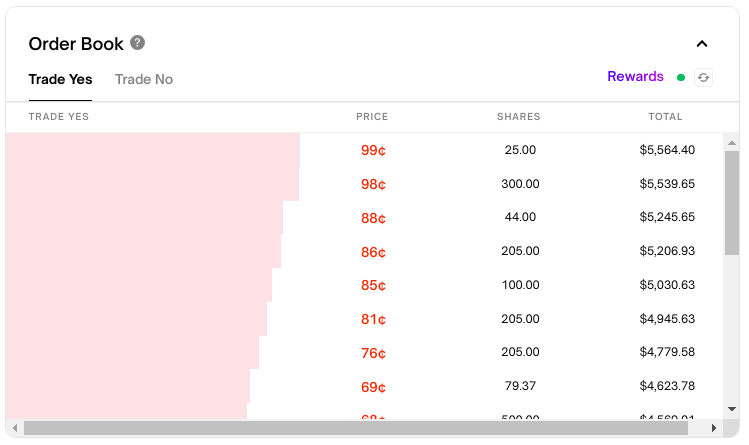
\includegraphics[scale=0.3]{img/order_book_yes_ask.png}
        \caption{Order Book for the Long Position: Ask}
        \label{fig:order_book_yes_ask}
    \end{minipage}
\end{figure}

Orders in the Ask section are arranged such that those with the lowest price have priority. Conversely, orders in the Bid section are arranged  from the highest price to the lowest.
    
In both the Ask and Bid sections, agents set their prices according to the level of certainty they have that the contract will be executed in their favor. Buyers with low expectations are willing to enter the market only if the price of the share is low (Figure \ref{fig:order_book_yes_bid}). Conversely, sellers with high expectations are willing to leave the market only if the price of the share is high (Figure \ref{fig:order_book_yes_ask}).